\documentclass[11pt, a4paper]{report}
\usepackage{etoolbox}
\makeatletter
\patchcmd{\chapter}{\if@openright\cleardoublepage\else\clearpage\fi}{}{}{}
\makeatother
\usepackage[margin=1in]{geometry}
\usepackage[utf8]{inputenc} % Umožňuje psaní českých znaků
\usepackage[czech]{babel}   % Česká lokalizace pro babel
\usepackage{titlesec}
\usepackage{pdfpages}
\usepackage{tabularx}
\usepackage{xcolor}
\titleformat{\chapter}
  {\normalfont\LARGE\bfseries}{\thechapter}{1em}{}
\titlespacing*{\chapter}{0pt}{3.5ex plus 1ex minus .2ex}{2.3ex plus .2ex}
\begin{document}
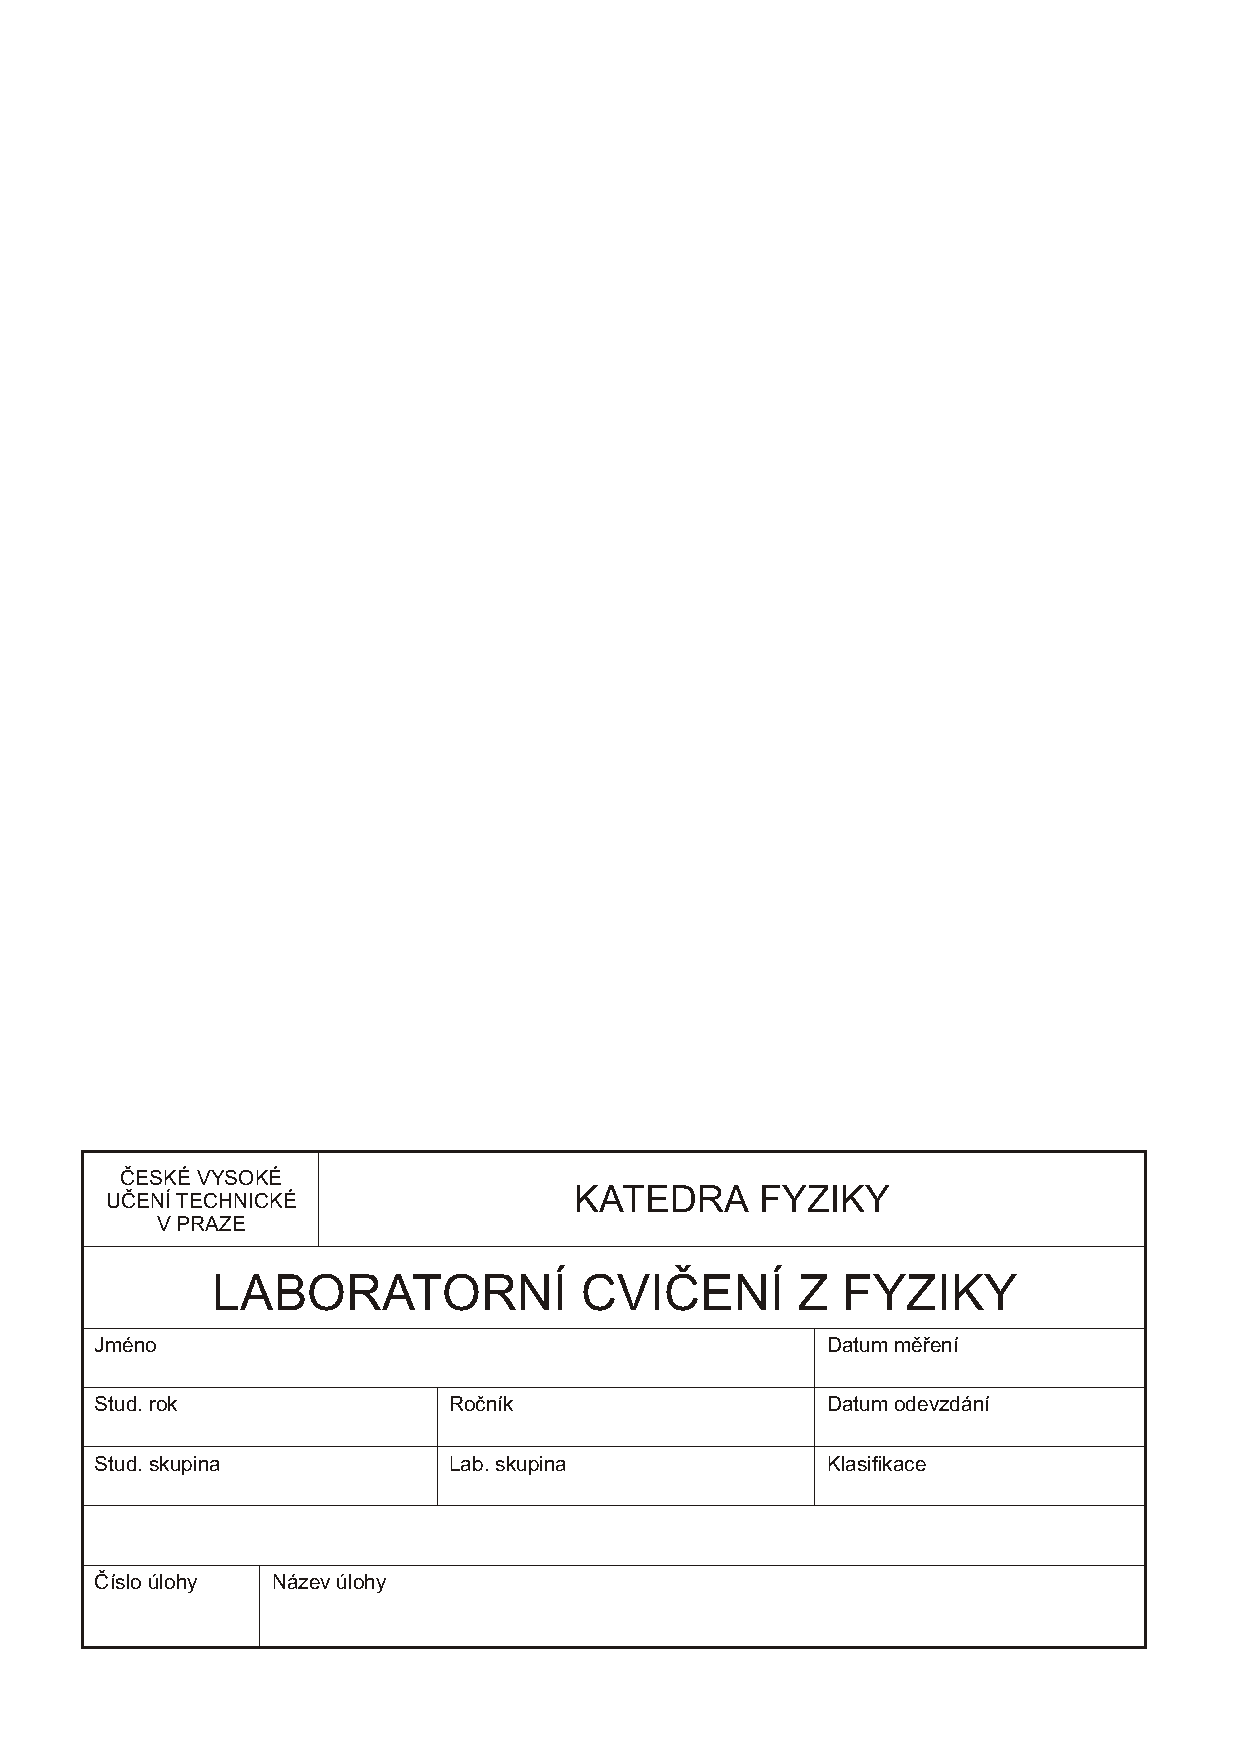
\includepdf{stamp.pdf}
\chapter{Úkol měření}
\begin{enumerate}
	\item Změřit objem válce
	\item Vypočítat \emph{kombinovanou standardní nejistotu} jednotlivých charakteristických rozměrů zkoumaného válce
	\item Vypočítat \emph{kombinovanou standardní nejistotu} objemu celého válce
\end{enumerate}
\vspace{5ex}
\chapter{Seznam použitých přístrojů}
\begin{center}
	\begin{tabularx}{1 \textwidth}{
			| >{\centering\arraybackslash}X
			| >{\centering\arraybackslash}X
			| >{\centering\arraybackslash}X |}
		\hline
		\bf{Měřící přístroj} & \bf{Identifikační číslo} & \bf{Přesnost} \\
		\hline
		\hline
		Posuvné měřidlo      & číslo neznámé            & 20 \mu m      \\
		\hline
		Mikrometr            & číslo neznámé            & 10 \mu m      \\
		\hline
	\end{tabularx}


\end{center}

\chapter{Naměřené hodnoty a výpočet}
\begin{center}
	\renewcommand{\arraystretch}{1.5}
	\begin{tabularx}{0.8 \textwidth}{
		| >{\centering\arraybackslash}m{2cm}
		| >{\centering\arraybackslash}X
		| >{\centering\arraybackslash}X|}
		\hline
		\bf{měření}   & \bf{d [mm] měřeno mikrometrem} & \bf{h [mm] měřeno pos. měřidlem} \\
		\hline
		\bfseries 1.  & 19,96                          & 15,92                            \\ \hline
		\bfseries 2.  & 19,97                          & 15,90                            \\ \hline
		\bfseries 3.  & 19,96                          & 15,88                            \\ \hline
		\bfseries 4.  & 19,97                          & 15,90                            \\ \hline
		\bfseries 5.  & 19,97                          & 15,88                            \\ \hline
		\bfseries 6.  & 19,96                          & 15,90                            \\ \hline
		\bfseries 7.  & 19,96                          & 15,78                            \\ \hline
		\bfseries 8.  & 19,96                          & 15,90                            \\ \hline
		\bfseries 9.  & 19,96                          & 15,88                            \\ \hline
		\bfseries 10. & 19,97                          & 15,92                            \\ \hline
	\end{tabularx}
\end{center}
\clearpage
\noindent Aritmetický průměr naměřených hodnot: \newline

\Large\[\overline{d} = \frac{1}{n}\sum_{i=1}^{n}d_i \doteq 19,96\,mm\;;\;\overline{h} = \frac{1}{n}\sum_{i=1}^{n}h_i \doteq 15,89\,mm\]
\normalsize
\newline Výpočet nejpravděpodobnější hodnoty objemu válce: \newline
\Large\[\overline{V} = \frac{1}{4}\pi\overline{d}^2\overline{h} \doteq 4 972,78\,mm^3\]
\normalsize
\newline Výpočet standardní nejistoty aritmetického průměru meřených hodnot metodou typu A:
\Large\[u_A(\overline{d})= \sqrt{\frac{1}{n(n-1)}\sum_{i=1}^{n}(d_i - \overline{d})^2} \doteq 0,00163299\,mm\]
\[u_A(\overline{h})= \sqrt{\frac{1}{n(n-1)}\sum_{i=1}^{n} (h_i - \overline{h})^2} \doteq 0,01266667\,mm\]
\normalsize
\newline
\noindent Výpočet standardní nejistoty nameřených hodnot metodou typu B:
\Large\[\Delta_d = 10\, \mu m = 0,01\,mm\;;\;\Delta_h = 20\, \mu m = 0,02\,mm\]
\[u_B(\Delta_d) = \frac{\Delta_d}{\sqrt{12}} \doteq 0,00288675\,mm\;;\;u_B(\Delta_h) \doteq \frac{\Delta_h}{\sqrt{12}} = 0,00577350\,mm\]
\newline
\normalsize Výpočet kombinované standardní nejistoty:
\Large\[u_c(\overline{d}) = \sqrt{u_{Ad}^2 + u_{Bd}^2}\doteq0,00329988\,mm\]
\[u_c(\overline{h}) = \sqrt{u_{Ah}^2 + u_{Bh}^2}\doteq  0,01392041\,mm\]
\normalsize
\newline
\noindent Výpočet kombinované standardní nejistoty objemu celého válce:
\Large\[u_c(\overline{V}) = \sqrt{\frac{\pi^2\overline{d}^2}{16}u_c^2(\overline{h})+ \frac{\pi^2\overline{d}^2\overline{h}^2}{4}u_c^2(\overline{d})} \doteq 1,62\,mm^3\]


\chapter{Závěr}
\normalsize Měřením válce bylo zjištěno, že jeho objem je (4972,78 \pm\:1,62) [mm\textsuperscript{3}].
\end{document}